\section{Leader election}
The objective of the leader election algorithm is to get a set of processes to elect a single leader. A leader has to keep track of all nodes in the system. The prerequisite is that all participating processes can lead and call for an election.

\subsection{Relevance in distributed systems}
In distributed systems a leader role is often designated to a single node/process. This node will often have the responsibility to coordinate, initiate and assign processing and tasks to the other nodes in the distributed system; and this is an attractive feature, since it eases synchronization, communication and delegation.
However, a leader is a single point of failure, and therefore the system needs to be prepared to reselect a new leader.
Leader election is the process of selecting this leader, both when initiating the system, and when a leader fails.
This is often difficult, since all nodes in the system has to cooperate, and elect the appropriate new leader.

\subsection{Burden}
If not handled correctly, leader election can draw a significant amount on both processing power and network, which results in a waste of resources and a slower distributed system. Algorithms can optimize efficiency and time used for a leader election, by minimizing messages sent between nodes on the network.
By minimizing the potential burden on network, time and computation the system will become both faster and more effective.
The big O notation can be used to analyze an algorithms complexity. By analyzing the amount of messages passed in the system for each algorithm, we can choose the most appropriate one and hereby reduce the burden on the system.

\subsection{Algorithm}

\subsubsection{Bully election algorithm}
When a process notices that the coordinator\footnote{Interchangeable with leader} unexpectedly crashes and/or no longer responding to its requests, it initiates an election.
During the election phase, the process which holds the election, will notify by sending an ELECTION message, only to processes with higher ID numbers than its own.

At any moment a process can receive an ELECTION message from one of its own lower-numbered colleagues, and when such a message is received, it will respond back to the sender with an OK message to indicate that it is alive and will then hold the election, unless it is already holding one.

The election phase finishes after, a repetition of sending and holding the election, till the one process with the highest ID number holds the election.

The winner of the election is the one process with the highest ID number, and will be taken over the role as the new coordinator, and notifies all other processes with a message stating its role as the new coordinator.

At any given time, when a process which had a downtime becomes operational, it will hold the election.
And yet again, the election phase will finish till the one process with highest ID number holds the election. So if the awaken process happens to have the highest ID number of all processes, it will become the winner of the election and take over the role as the coordinator. Hence the name “Bully election” because the one who plays the game right is also the one who sits on the throne.

\subsubsection{Bully election algorithm}
In order for this algorithm to make sense, an assumption has to be made, that the processes has to be either physically or logically ordered, so that each process is able to identify its successor.

When a process notices that the current coordinator for some reason is not operational, it will send out an ELECTION message, which in the message contains the process own ID number. The message will be sent to its successor.

If the successor is down, the sender skips over the broken successor, and persist the message to the next member according to the ordering. The receiver of the message will then add its own ID number to the list and send it to its successor. This is repeated till it gets back to the original process which started the circulation of message, which is identified by the list of ID numbers.

The original sender of the ELECTION message will then change the type of message from ELECTION to COORDINATOR, and circulate the message yet again, but this time, the message is responsible:

\begin{itemize}
  \item Stating that the one with the highest ID number in the list, is the new coordinator
  \item Update the ring with processes which is alive and functional upon ELECTION phase
\end{itemize}

When the message has been circulated around to all members from the list, the election phase finishes and the system resume its work.

\subsubsection{Improved version of Bully election algorithm}

Bully election algorithm is simple and fault tolerant, and therefore commonly used in a distributed system. Considering the algorithm, for each process in a system, there is a high occurrence of message passing between processes during the election phase, which results in a higher traffic on the communication channels, and will be amplified with queuing due to traffic overflow. In short the Bully election algorithm is prone to a higher response time within a distributed system.

The classic Bully election algorithm has another flaw. Consider a situation where a process that is designated as the coordinator unexpectedly becomes unavailable and out of function, which results in an election phase as mentioned earlier.

During the election phase, a process joins the group and becomes part of the election phase and also happens to be a higher-numbered process than the previous coordinator. It will therefore also take the role as the new coordinator and the system resumes its ongoing job.

Consider the event, where the previous coordinator becomes available again, and the election phase will occur yet again, and it will elect itself as the new coordinator because it has no update on the newly joined process that also happens to be a higher numbered process. There will be 2 coordinators; one of them is neglected and is not being reached, and this faulty will persist till a new election phase begins.
To overcome this situation, an alternative to the classic Bully election algorithm, can be implemented, and is named Fast Bully election algorithm.

In short what it does to overcome the situation where another process joins the group of processes, is to add different types of message, but in this case, a view message is introduced.
What it does it that when a process is recovered from the downtime, it will also receive a view message that updates all processes in the group and also those newly joined.

The figure propose the difference between the classic Bully Algorithm to the Fast Bully Algorithm with use of Big O notation.


\begin{figure}[ht]
\centering
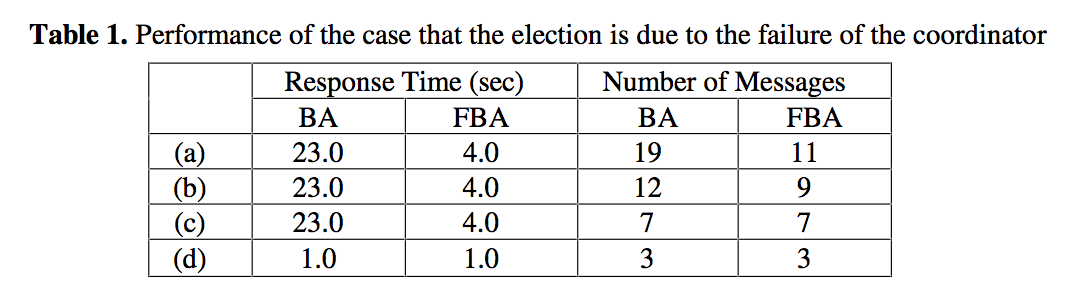
\includegraphics[width=100mm]{img/big_o_notation_overview_for_BA.png}
\caption{Difference between Bully Algorithm and Fast Bully Algorithm with use of big o notation}
\end{figure}


